\documentclass[a4paper]{article}
\usepackage[T2A]{fontenc}            % Поддержка русских букв
\usepackage[utf8]{inputenc}          % Кодировка utf8
\usepackage[english, russian]{babel} % Языки: английский, русский
\usepackage[a4paper, left=2.5cm, right=1.5cm, top=2.5cm, bottom=2.5cm]{geometry}
\usepackage{graphicx}
\graphicspath{{pictures/}}
\DeclareGraphicsExtensions{.pdf,.png,.jpg}

\begin{document}
\title{``Разгон'' резисторов}
\author{В.В. Некрасов}
\date{\today}
\maketitle

\section{Цель}

    В ГОСТ 24238-84 ~\cite{gost24238-84} п. 2.3.4.4. сказано, что резисторы должны выдерживать воздействие импульсной нагрузки. Параметры
допустимой импульсной нагрузки должны быть указаны в стандартах или ТУ на резисторы конкретных типов. Однако
в этих стандартах и ТУ обычно нормируется допустимая мощность для импульса одной длительности.

	Попробуем с помощью термодинамики определить зависимость допустимой мощности от длительности импульса.
Недостатком этой оценки является невозможность учесть влияние местных перегревов, вызывающих постепенную
деградацию.

\section{Уравнение нагревания}

    Предположим, что резисторы обладают равномерным рассеиванием тепла со всей поверхности и бесконечно
большой теплопроводностью.

    Также предположим, что вся подводимая мощность превращается в тепло $Q$. Эта теплота частично
аккумулируется в теле резистора, повышая его температуру, частично отдаётся во внешнюю среду.

    При аккумулировании мощности за время $dt$ потребляется энергия $Q{\cdot}dt$. Это приводит к разогреву
тела резистора. Величина изменения температуры $d{{\Theta}}=\frac{Q{\cdot}dt}{G{\cdot}c}$, где $G$ - масса
тела, $C$ - его удельная теплоёмкость.

    Разность температуры ${\Theta}$ между телом и окружающей средой вызывает теплообмен. Количество
теплоты $Q$, отдаваемое в окружающее пространство за время dt будет
$Q{\cdot}dt=S{\cdot}{\lambda}{\cdot}{\Theta}{\cdot}dt$, где $S$-площадь тела, ${\lambda}$-коэффициент
теплопередачи.

    Тогда:
\begin{equation}
\label{e_balance}
Q{\cdot}dt=G{\cdot}c{\cdot}d{\Theta}+S{\cdot}{\lambda}{\cdot}{\Theta}{\cdot}dt
\end{equation}

\section{Установившаяся температура и постоянная времени нагревания}

    Когда пройдёт бесконечное время температура тела достигнет установившегося
значения. Тогда $d{\Theta}=0$ и ${\Theta}={\Theta}_\infty$. Подставив эти значения в
выражение (\ref{e_balance}). Получим:

\begin{equation}
Q{\cdot}dt=S{\cdot}{\lambda}{\cdot}{\Theta}_{\infty}{\cdot}dt
\end{equation}

откуда:

\begin{equation}
\label{inf_temp}
{\Theta}_{\infty}=\frac{Q}{S{\cdot}{\lambda}}
\end{equation}

разделим обе части выражения (\ref{e_balance}) на $S{\cdot}{\lambda}$.

\begin{equation}
\frac{Q}{S{\cdot}{\lambda}}{\cdot}dt=\frac{G{\cdot}c}{S{\cdot}{\lambda}}{\cdot}d{\Theta}+{\Theta}{\cdot}dt
\end{equation}

подставим (\ref{inf_temp})

\begin{equation}
{\Theta}_{\infty}{\cdot}dt=\frac{G{\cdot}c}{S{\cdot}{\lambda}}{\cdot}d{\Theta}+{\Theta}{\cdot}dt
\end{equation}

обозначим

\begin{equation}
T=\frac{G{\cdot}c}{S{\cdot}{\lambda}}
\end{equation}

и получим

\begin{equation}
\label{heating}
{\Theta}_{\infty}{\cdot}dt=T{\cdot}d{\Theta}+{\Theta}{\cdot}dt
\end{equation}

Величина $T$ имеет размерность времени. Она называется \textbf{постоянной времени}.

\section{Решение уравнения нагревания}

Перепишем уравнение (\ref{heating}) в виде:

\begin{equation}
\label{new_heating}
\frac{dt}{T}=\frac{d\Theta}{\Theta_{\infty}-\Theta}
\end{equation}

Проинтегрировав по времени получим:

\begin{equation}
\label{integrated}
\frac{t}{T}=-\log{(\Theta_{\infty}-\Theta)}+C
\end{equation}

Постоянная $C$ определяется из начального условия: при $t=0$ имеем
$\Theta=\Theta_{0}$. Подставив в (\ref{integrated}) найдём:

\begin{equation}
    C=\log{(\Theta_{\infty}-\Theta_{0})}
\end{equation}

Подставим это значение $C$ в (\ref{integrated}).

\begin{equation}
\log{\frac{\Theta_{\infty}-\Theta}{\Theta_{\infty}-\Theta_{0}}}=-\frac{t}{T}
\end{equation}

Выразим $\Theta$:

\begin{equation}
    \Theta_{(t)} = \Theta_{\infty}{\cdot}(1-e^{-\frac{t}{T}}) +
         {\Theta}_{0}{\cdot}e^{-\frac{t}{T}}
\end{equation}

Для упрощения расчётов примем начальную температуру за $0$. Тогда $\Theta$
и $\Theta_\infty$ будут иметь значения превышения над начальной температурой.
Уравнение упрощается:

\begin{equation}
\label{final_eq}
\Theta_{(t)} = \Theta_{\infty}{\cdot}(1-e^{-\frac{t}{T}})
\end{equation}

Это уравнение показывает зависимость температуры от времени при подаче постоянной
мощности. Из (\ref{inf_temp}) видно что $\Theta_{\infty}$ пропорциональна подводимой
мощности.

Обозначим допустимую температуру как $\Theta_{nom}$. Перепишем (\ref{final_eq}) для
$\Theta_{\infty}=\Theta_{nom}{\cdot}q$

\begin{equation}
\label{overpowered_eq}
\Theta_{(t)} = \Theta_{nom}{\cdot}q{\cdot}(1-e^{-\frac{t}{T}})
\end{equation}

Но температура не должна превышать $\Theta_{nom}$. Тогда:

\begin{equation}
\label{overpowered_eq}
\Theta_{nom} = \Theta_{nom}{\cdot}q{\cdot}(1-e^{-\frac{t}{T}})
\end{equation}

Теперь можем узнать за какое время достигается $\Theta_{ном}$ при
$\Theta_{\infty}=\Theta_{nom}{\cdot}q$.

\begin{equation}
\label{tpulse_eq}
    t_{(q)} = -T{\cdot}log(1-\frac1q)
\end{equation}

\section{Исходные данные}

	В АЛЯР.434110.005 ТУ-ЛУ \cite{alyr.434110.005} резисторов Р1-12-0,25 в п.
4.3.6.2 рисунке 2 показано, что предельная температура работы этих резисторов равна
$155^{\circ}$. Можно предположить, что при импульсном режимах определённых в п.
4.3.6.5 достигается такая же температура. Тогда допустимый перегрев резистора от
максимальной рабочей температуры $155-50=105^{\circ}$. Т.е. при коэффициенте
перегрузке $q=20$ и длительности импульса в 1000 мкс достигнет предельной температуры.

    Из ($\ref{inf_temp}$) видно, что температура в установившемся режиме
${\Theta}_{\infty}$ пропорциональна подводимой мощности.

    Подставляем эти данные в ($\ref{final_eq}$)

\begin{equation}
105 = 105{\cdot}20{\cdot}(1-e^{-\frac{1{\cdot}10^{-3}}{T}})
\end{equation}

    Получаем значение постоянной времени $T$ резисторов Р1-12-0,25 в секундах.

\begin{equation}
T=\frac{1}{\log{(1-\frac{1e-3}{20})}}=19,5{\cdot}10^{-3}
\end{equation}

%     Тогда температура при такой перегрузке будет рости по такому закону.
% 
% \begin{equation}
% \Theta_{(t)} = 105{\cdot}20{\cdot}(1-e^{-\frac{t}{19,5{\cdot}10^{-3}}})
% \end{equation}

    Теперь можно узнать зависимость допустимой мощности от длительности импульса.

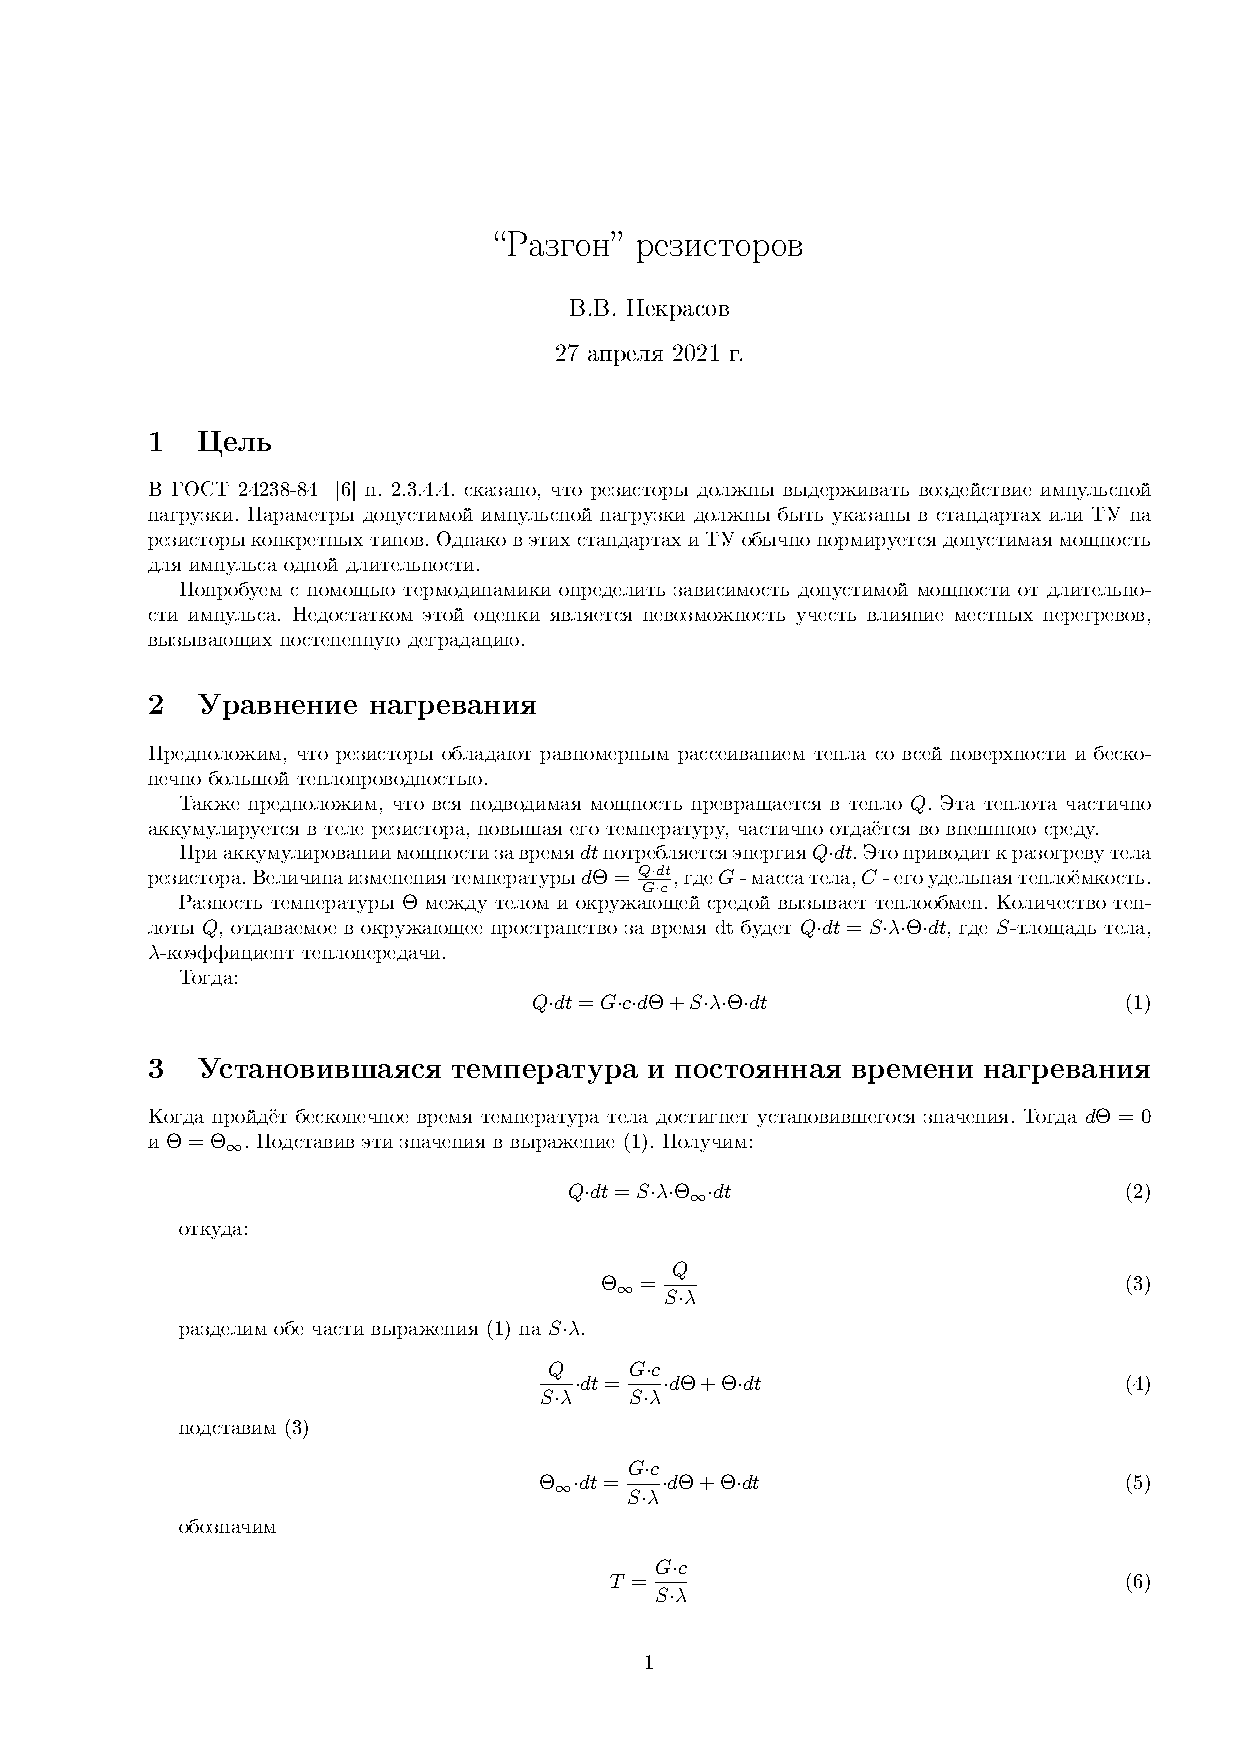
\includegraphics{Overclocking_resistors.png}

\begin{thebibliography}{2}
\bibitem{alyr.434110.005}
    Резисторы постоянные непроволочные Р1-12. Технические условия АЛЯР.434110.005 ТУ

\bibitem{0j0.467.093}
    Резисторы постоянные непроволочные С2-33. Технические условия ОЖО.467.093 ТУ

\bibitem{0j0.467.089}
    Резисторы постоянные непроволочные С2-36. Технические условия ОЖО.467.089 ТУ

\bibitem{0j0.467.531}
    Резисторы постоянные непроволочные С5-47. Технические условия ОЖО.467.531 ТУ

\bibitem{gost21342.14-86}
    Резисторы методы испытания импульсной нагрузкой ГОСТ 21342.14-86

\bibitem{gost24238-84}
    Резисторы постоянные общие технические условия ГОСТ 24238-84

\bibitem{heating_cooling}
    Нагревание и охлаждение идеального однородного твердого тела.
URL: https://www.electromechanics.ru/direct-current/591-heating-and-cooling-is-ideal-homogeneous-solid.html
\end{thebibliography}

\end{document}
